\documentclass[border=4pt,12pt]{standalone}
% House style for redrawn exam diagrams (diagram-v4: 0.4pt lines, filled -latex arrows, fine dashes; stipple and hatching drawn as real dots/lines (no PDF/SVG patterns, so they render in every browser and at any scale); transparent background). Every figure \input's this.
\usepackage{amsmath,amssymb}
\usepackage{txfonts}
\usepackage{pdfrender,xcolor}
% \halo{text}: label on shading. The shading stops just around each letter's outline (a thin knock-out that follows the
% glyphs, like the papers' typesetting), never a box. Owner: "I don't want a box around the text".
\newcommand{\halo}[1]{\leavevmode\rlap{\pdfrender{TextRenderingMode=2,LineWidth=2.2pt,LineJoinStyle=1,StrokeColor=white,FillColor=white}#1}#1}
\usepackage{tikz,pgfplots}
\pgfplotsset{compat=1.18}
\usetikzlibrary{arrows.meta,calc,angles,quotes,patterns,patterns.meta,intersections,positioning,decorations.markings,shapes.geometric}
% Stipple and hatching are drawn as actual dots / lines clipped to the region (path picture), NOT as pattern fills:
% SVG <pattern> fills vanish or blur when browsers scale the image, so the owner could not see the shading.
% Each dot is a 0.72pt square (keeps SVGs small; reads as a dot at print size). Dots sit on one global staggered grid, so neighbouring regions line up.
\makeatletter
\newdimen\ex@x \newdimen\ex@y \newdimen\ex@xa \newdimen\ex@ya \newdimen\ex@xb \newdimen\ex@yb \newcount\ex@row
\def\exam@stipplecolor{black!75}\def\exam@dotr{0.42pt}\def\exam@dotgap{2.5}
\def\ex@rowdots{\ifdim\ex@x<\ex@xb \pgfpathrectangle{\pgfqpoint{\dimexpr\ex@x-0.36pt\relax}{\dimexpr\ex@y-0.36pt\relax}}{\pgfqpoint{0.72pt}{0.72pt}}\advance\ex@x by \exam@dotgap pt\relax\expandafter\ex@rowdots\fi}
\def\exam@stipple{%
  \pgftransformreset% dots are sized in real points even inside scaled pictures
  \pgfpointanchor{path picture bounding box}{south west}\ex@xa=\pgf@x \ex@ya=\pgf@y
  \pgfpointanchor{path picture bounding box}{north east}\ex@xb=\pgf@x \ex@yb=\pgf@y
  \pgfsetfillcolor{\exam@stipplecolor}\pgfmathsetmacro\ex@h{\exam@dotgap/2}%
  \pgfmathtruncatemacro\ex@r{floor(\ex@ya/\ex@h)-1}\ex@row=\ex@r\relax
  \ex@y=\ex@r\dimexpr\ex@h pt\relax
  \loop\ifdim\ex@y<\ex@yb
    \pgfmathtruncatemacro\ex@c{floor(\ex@xa/\exam@dotgap)-1}\ex@x=\ex@c\dimexpr\exam@dotgap pt\relax
    \ifodd\ex@row \advance\ex@x by \ex@h pt\fi
    \ex@rowdots
    \advance\ex@y by \ex@h pt \advance\ex@row by 1
    \ifnum\numexpr\ex@row-(\ex@row/4)*4\relax=0 \pgfusepath{fill}\fi% flush every 4 rows: bounded TeX memory, few clip copies in the SVG
  \repeat\pgfusepath{fill}}
\newdimen\ex@d
\def\exam@hatch#1{% #1 = 1 for /, -1 for \ ; lines 45 degrees, 3pt apart
  \pgftransformreset
  \pgfpointanchor{path picture bounding box}{south west}\ex@xa=\pgf@x \ex@ya=\pgf@y
  \pgfpointanchor{path picture bounding box}{north east}\ex@xb=\pgf@x \ex@yb=\pgf@y
  \ex@d=\dimexpr\ex@yb-\ex@ya\relax \ex@x=\dimexpr\ex@xa-\ex@d\relax
  \loop\ifdim\ex@x<\ex@xb
    \ifnum#1>0 \pgfpathmoveto{\pgfqpoint{\ex@x}{\ex@ya}}\pgfpathlineto{\pgfqpoint{\dimexpr\ex@x+\ex@d\relax}{\ex@yb}}%
    \else \pgfpathmoveto{\pgfqpoint{\ex@x}{\ex@yb}}\pgfpathlineto{\pgfqpoint{\dimexpr\ex@x+\ex@d\relax}{\ex@ya}}\fi
    \advance\ex@x by 4.24pt
  \repeat
  \pgfsetlinewidth{0.4pt}\pgfsetstrokecolor{black}\pgfusepath{stroke}}
\def\examstipple{\exam@stipple}\def\examhatch{\exam@hatch}\def\examsetstipplecolor#1{\def\exam@stipplecolor{#1}}\def\examsetdotgap#1{\def\exam@dotgap{#1}}
\makeatother
% (legacy pattern kept for old files)
% staggered stipple like the NESA papers' dotted shading
\pgfdeclarepatternformonly{exam stipple}{\pgfpointorigin}{\pgfqpoint{2.2pt}{2.2pt}}{\pgfqpoint{2.2pt}{2.2pt}}{%
  \pgfpathcircle{\pgfqpoint{0.55pt}{0.55pt}}{0.42pt}\pgfpathcircle{\pgfqpoint{1.65pt}{1.65pt}}{0.42pt}\pgfusepath{fill}}
\tikzset{
  every picture/.style={line width=0.6pt, >={Latex[length=2mm,width=1.3mm]}},
  curve/.style={line width=0.6pt},
  open arrow/.style={-{Latex[length=2mm,width=1.3mm]}},  % owner: filled -latex heads everywhere, no open chevrons
  aux/.style={dash pattern=on 2pt off 1.5pt, line width=0.6pt},
  shade/.code={\def\exA{#1}\def\exB{none}\ifx\exA\exB\else\pgfkeysalso{fill=black!18}\fi},
  shade/.default=on,
  shade dots/.style={fill=none, path picture={\examstipple}},
  stipple color/.code={\examsetstipplecolor{#1}},
  stipple gap/.code={\examsetdotgap{#1}},
  shade dense dots/.style={fill=none, stipple gap=1.6, path picture={\examstipple}},
  shade hatch/.style={fill=none, path picture={\examhatch{1}}},
  shade hatch reverse/.style={fill=none, path picture={\examhatch{-1}}},
  shade solid/.style={fill=black},
  pt/.style={circle, fill, inner sep=1.1pt},
  open pt/.style={circle, draw, fill=white, inner sep=1.1pt},
}
\pgfplotsset{
  exam axes/.style={axis lines=middle, axis line style={->}, xlabel={$x$}, ylabel={$y$},
    xlabel style={anchor=west}, ylabel style={anchor=south}, tick label style={font=\small},
    every axis plot/.append style={line width=0.6pt, black}, samples=200, clip=false,
    enlargelimits=false, axis on top},
}

\begin{document}
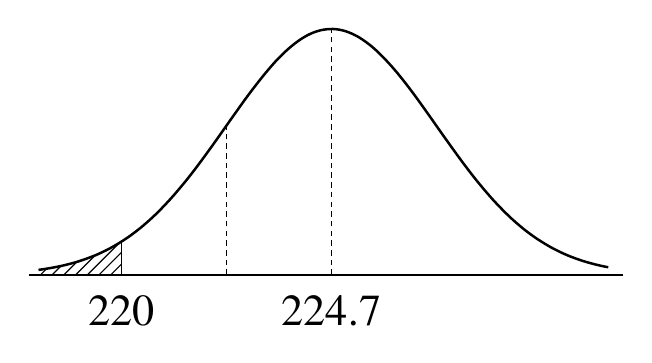
\begin{tikzpicture}[x=0.0127cm,y=-0.0127cm,font=\fontsize{16}{19.2}\selectfont]
\path[shade hatch] (10,276.0) -- plot[smooth] coordinates {(10.0,271.0) (12.8,270.6) (15.5,270.2) (18.3,269.8) (21.1,269.3) (23.8,268.8) (26.6,268.3) (29.4,267.8) (32.1,267.2) (34.9,266.6) (37.7,265.9) (40.4,265.2) (43.2,264.5) (46.0,263.7) (48.7,262.9) (51.5,262.0) (54.3,261.1) (57.0,260.2) (59.8,259.2) (62.6,258.1) (65.3,257.0) (68.1,255.9) (70.9,254.6) (73.6,253.4) (76.4,252.0) (79.2,250.6) (81.9,249.2) (84.7,247.7) (87.5,246.1) (90.2,244.4) (93.0,242.7)} -- (93.0,276.0) -- cycle;
\draw (93.0,276.0)--(93.0,242.7);
\draw (0,276.0)--(595,276.0);
\draw[line width=0.9pt] plot[smooth] coordinates {(10.0,271.0) (16.4,270.1) (22.8,269.0) (29.2,267.8) (35.6,266.4) (42.0,264.8) (48.4,263.0) (54.8,260.9) (61.2,258.6) (67.6,256.1) (74.0,253.2) (80.4,250.0) (86.9,246.4) (93.3,242.5) (99.7,238.3) (106.1,233.6) (112.5,228.6) (118.9,223.1) (125.3,217.3) (131.7,211.0) (138.1,204.3) (144.5,197.3) (150.9,189.8) (157.3,182.1) (163.7,174.0) (170.1,165.6) (176.5,156.9) (182.9,148.1) (189.3,139.1) (195.7,130.0) (202.1,120.9) (208.5,111.9) (214.9,102.9) (221.3,94.2) (227.8,85.7) (234.2,77.6) (240.6,69.9) (247.0,62.6) (253.4,56.0) (259.8,50.0) (266.2,44.7) (272.6,40.1) (279.0,36.3) (285.4,33.4) (291.8,31.4) (298.2,30.3) (304.6,30.0) (311.0,30.7) (317.4,32.3) (323.8,34.8) (330.2,38.1) (336.6,42.3) (343.0,47.2) (349.4,52.9) (355.8,59.3) (362.2,66.2) (368.7,73.7) (375.1,81.6) (381.5,89.9) (387.9,98.5) (394.3,107.4) (400.7,116.4) (407.1,125.5) (413.5,134.6) (419.9,143.6) (426.3,152.5) (432.7,161.3) (439.1,169.8) (445.5,178.1) (451.9,186.0) (458.3,193.6) (464.7,200.9) (471.1,207.7) (477.5,214.2) (483.9,220.3) (490.3,225.9) (496.7,231.2) (503.1,236.0) (509.6,240.5) (516.0,244.5) (522.4,248.3) (528.8,251.6) (535.2,254.7) (541.6,257.4) (548.0,259.8) (554.4,262.0) (560.8,263.9) (567.2,265.6) (573.6,267.1) (580.0,268.4)};
\draw[aux] (303.0,276.0)--(303.0,30.0);
\draw[aux] (198.0,276.0)--(198.0,126.8);
\node at (93.0,312) {$220$};
\node at (303.0,312) {$224.7$};\end{tikzpicture}
\end{document}
